\documentclass{article}
\usepackage[utf8x]{inputenc}
\usepackage{lipsum}
\usepackage[margin=1in,includefoot]{geometry}
\usepackage{fancyhdr}
\pagestyle{fancy}
\usepackage{pifont}
\newcommand{\cmark}{\ding{51}}
\newcommand{\xmark}{\ding{55}}
\usepackage{listings}
\usepackage{color}
\usepackage{hyperref}
\usepackage[table]{xcolor}
\usepackage{graphicx}
\usepackage{float}
\usepackage{longtable}
\usepackage[T1]{fontenc}
\usepackage{textcomp}
\usepackage[english]{babel}
\usepackage[T1]{fontenc}
\usepackage{uarial}
\renewcommand{\familydefault}{\sfdefault}
\definecolor{dkgreen}{rgb}{0,0.6,0}
\definecolor{gray}{rgb}{0.5,0.5,0.5}
\definecolor{mauve}{rgb}{0.58,0,0.82}
\hypersetup{
    colorlinks=true, % make the links colored
    linkcolor=black, % color TOC links in blue
    urlcolor=blue, % color URLs in red
    linktoc=all % 'all' will create links for everything in the TOC
}
\lstset{
    commentstyle = \color{gray},
    extendedchars = \true,
    inputencoding = utf8x,
    language = php,
    keepspaces = true,
    keywordstyle = \bfseries,
    backgroundcolor = \color{blue!25},
    xleftmargin = 2cm,
    framexleftmargin = 1em
}

\begin{document}
\rowcolors{2}{teal!20}{white}
\begin{titlepage}
\begin{center}
\begin{figure}[H]
\centering

\includegraphics[width=2.8 in]{306.png}
\end{figure}
\line(1,0){350}\\
\huge{\bfseries Zaakpay Integration Document}
\line(1,0){250}\\
[1.5cm]
\textsc{\Large Version 2.0}
\end{center}


\end{titlepage}
\thispagestyle{empty}
\tableofcontents
\thispagestyle{empty}
\newpage
\listoffigures
\listoftables
\thispagestyle{empty}
\cleardoublepage
\setcounter{page}{1}
\section{Introduction}\label{sec:Intro}
Zaakpay is an online payments platform that offers multiple payment methods to both an individual user and a business. 

So, whether you are an ecommerce giant, a small spunky start-up or an individual user simply wanting to make payments to businesses, we have products that cater to all your needs.

This document describes the steps for technical integration process between merchant website/app and Zaakpay Payment Gateway for enabling online transactions. This document is covered in two sections. Section 1 covers website integration and Section 2 covers the APIs provided to the merchants.

\section{Sign-Up}
Signup for a business account on Zaakpay. After signing up and verifying your account
follow the steps below:
\begin{itemize}
\item  Login to Zaakpay on \url{https://www.zaakpay.com}
\begin{figure}[H]
\centering
\caption{Sign-Up}
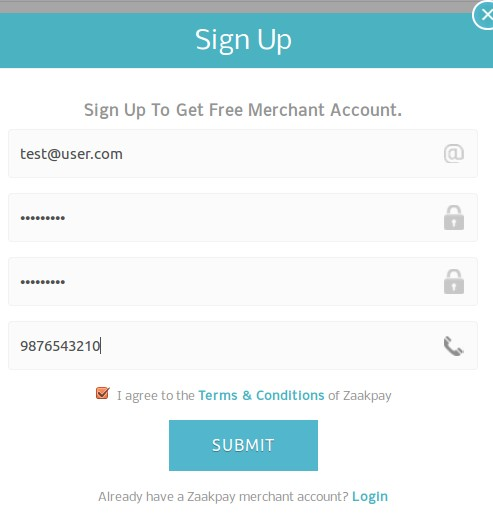
\includegraphics[width=0.8\textwidth,height=4.3in]{Signup1.png}
\end{figure}
\item  Click the My Account tab.
\item  Select the integration sub-menu item under the My Account tab.
\item   Select the URLs \& Keys tab from the navigation.
\item  Fill in details like the domain you'll be posting from and your return URL.Here the domain is the domain where you'll be posting data to Zaakpay from and the response URL for transact API is the path to the response.ext file on your server.
\item Select the Transaction limits sub-menu item under the My Account tab and set your appropriate transaction limits.
\end{itemize}
 \begin{figure}[H]
\centering
\caption{Dashboard-Home}
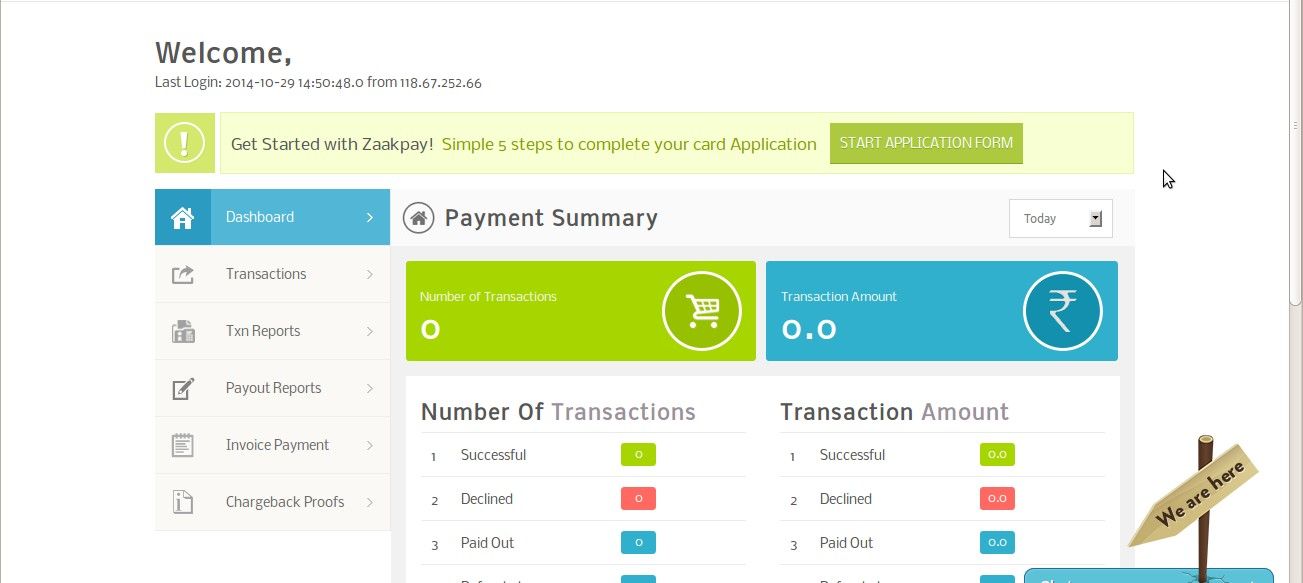
\includegraphics[width=1.1\textwidth,height=4.2in]{Zaakpay_panel.png}
\end{figure}
Generate your secret key and note it down along with your merchant identification
number.

\newpage
\section{Get Merchant ID and Secret Key}
Login to your Zaakpay account with registered email id. Go to Integration section. You’ll get your Merchant Identifier and Secret key in URLs and Keys section. \\
\begin{figure}[H]
\centering
\caption{Dashbaord-Developer Section}
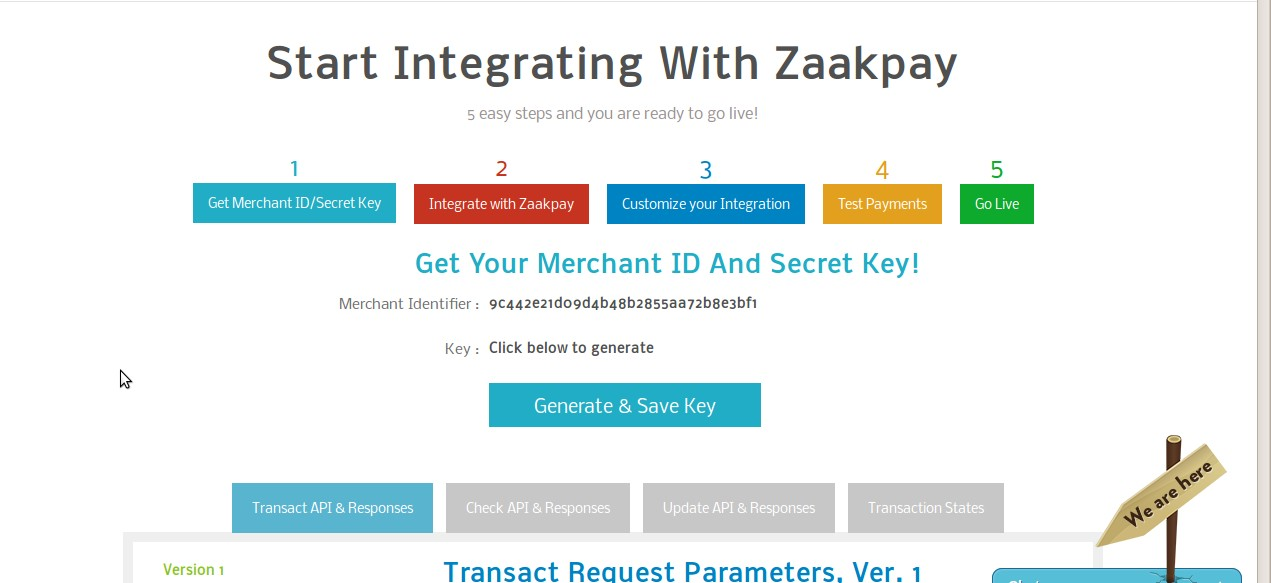
\includegraphics[width=1\textwidth,height=3.3in]{Zaakpay_panel1.png}
\end{figure}

If Secret key is blank, you can generate Key by pressing the button “Generate Key” and save. If you're using the integration kit, please replace the values of the secret key in the response.ext and posttozaakpay.ext files where ext=extension.

Next, you need to fill in the domain details in your Zaakpay account. For that, click on "Customize your Integration" and then, click on "URL's" as described in the screen below.

\begin{figure}[H]
\centering
\caption{Dashboard-URL Section}
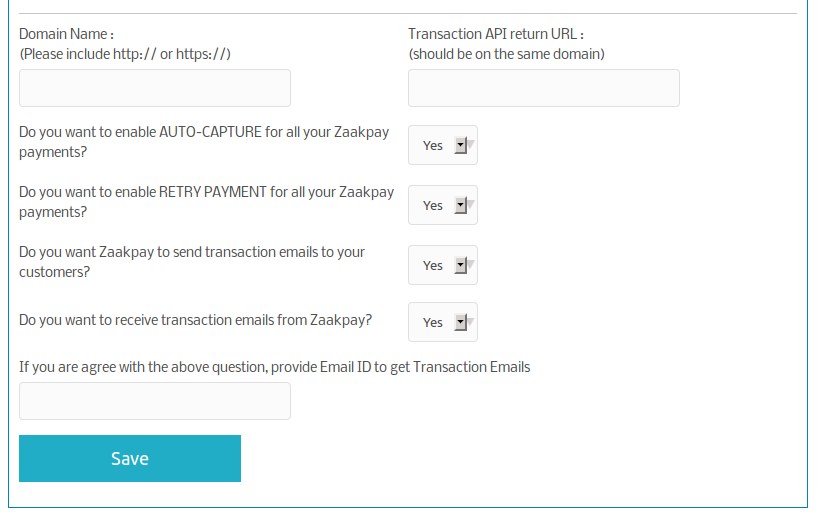
\includegraphics[width=0.8\textwidth,height=3.1in]{Data_not_complete.png}
\end{figure}

After this, proceed to the next tab, "Transaction Limits". Here you can update the transaction caps (upper and lower) as per your requirements.

\begin{figure}[H]
\centering
\caption{Dashboard-Transaction Limits}
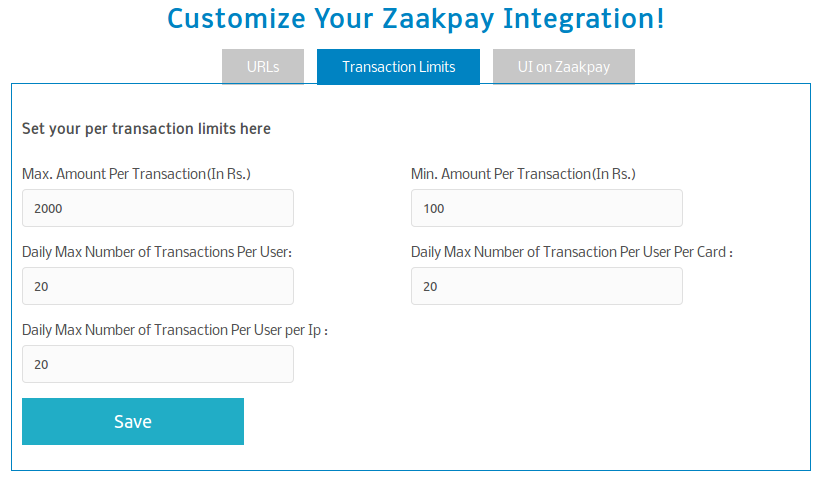
\includegraphics[width=0.8\textwidth,height=3.3in]{Transaction_limits.png}
\end{figure}

Next you can complete the integration UI by uploading a brand image on the ext tab.

\begin{figure}[H]
\centering
\caption{Dashboard-UI Section}
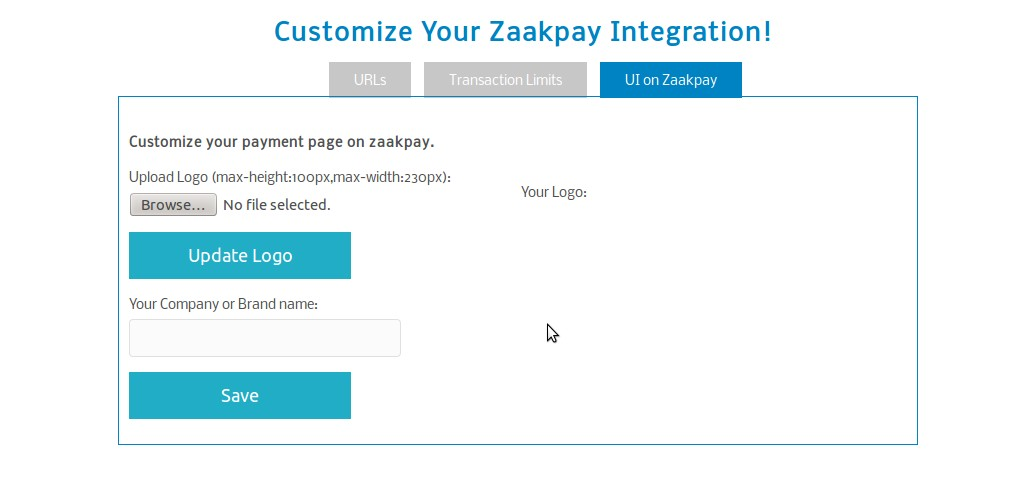
\includegraphics[width=0.8\textwidth,height=3.3in]{Zaakpay_ui.png}
\end{figure}
Click on "Save" once you are done with all these configurations.
\\

This was the overall set of procedures required for Zaakpay integration at our end. Next comes Merchant's side of integration, which is explained in the later sections.
\newpage
\section{Staging Credentials}
\begin{itemize}
\item {\bfseries URL : } http://zaakpay-staging.cloudapp.net:8080
\item {\bfseries Merchant Identifier :} b19e8f103bce406cbd3476431b6b7973
\item {\bfseries Secret key :} 0678056d96914a8583fb518caf42828a
\item {\bfseries Public KeyId :}
sAMtcgidueVcrZI
\item {\bfseries Public key :} MIIBIjANBgkqhkiG9w0BAQEFAAOCAQ8AMIIBCgKCAQEAikG2PaW+CqT3m\\26Dbtm7una22MYEDd+xONYjwE69Qa/FNQO0R5eqUnfi4lneWX6rc1IB6iVhyNDYULOZB\\W7vUsFbDWNJFDTD+V1T+30VXYvo+m7ufZCgxJVLn8W+JnKn1JPaL0n78UV2cG9zPlXK\\zJcMIGrNSG9QWFd6XJjlriJ2CFEbzPf7a4y7DwNgGrRpqMkmJDHNLcaba+CtTqjgeGUWo\\VIIg7RaQk4rJ5v21qyVK0pAUyfEXBDcLGWjsae0lsK+En7RFpV5NV6HxO78RnfT07RIdIBH\\xjWeM9WJ+xuGBKrODXmKRdWXSCAIiDYCp6F6fkgViE1XnCL6gQbnqQIDAQAB
\end{itemize}

\newpage
\section{Placing files on your server}
Based on your platform copy the posttozaakpay.ext, response.ext \& checksum.ext files on your server.Here .ext depends on the programming language your server is based on. 
\\
For example, for PHP the file names will be response.php, etc.
\begin{itemize}
\item Make sure the code at the top of the files posttozaakpay.ext and response.ext is pointing to correct path you’ve placed checksum.ext (In case of checksum.jar you need to place it where other jar files libraries are located.
\\ Example code :
\begin{lstlisting}[language=PHP]
// Hello.php
<%@ page import = ”com.zaakpay.lib.ChecksumCalculator” %>
<?php include(‘checksum.php’); ?>
\end{lstlisting}
\item Go to Zaakpay - My Account - Integration - URLs \& Keys and update your transact API Return URL to the path where response.ext file is on your website. 
\\Example:
http://yourbrandname.com/payment/response.jsp
\item In the response.ext file subject to the checksum validation process, you may use/store the response data as you see fit. A copy of this data will be available in the Transaction History section of the Zaakpay Merchant Dashboard.
\end{itemize}



\newpage

\section{Non Seamless Integration}
The purpose of this API is to enable websites to do online payment transactions using Zaakpay. Mobile Integration: For Zaakpay integration on mobile, parameter showMobile must be set to true. Everything else is same for desktop and mobile integration. 
\subsection{Checksum Calculation}
For both integrity \& data-authenticity verification before sending data to the API, you need to calculate a checksum of all the data that you send to Zaakpay. We use an HMACSHA- 256algorithm to calculate the checksum of ALL data that is posted to the API. We require data to be posted to our server in NVP (Name-Value Pairs) format.
\\ To calculate the checksum please follow the process below:
\begin{itemize}
\item Create a list of all parameters which you're passing to the API. Parameters used in checksum calculation are in the same order as the order of posting the parameters to Zaakpay.
\item Create a concatenated string of all data values in your list, with single quotes around each item. e.g. \textquotesingle{}merchantIdentifier\textquotesingle{}\textquotesingle{}orderId\textquotesingle{}\textquotesingle{}amount\textquotesingle{}\textquotesingle{}buyerEmail\textquotesingle{}\textquotesingle{}buyerAddress\textquotesingle{}...
\item Calculate the checksum using the HMAC SHA-256 algorithm using the concatenated string as data and your generated secret key.
\item The resulting checksum calculated should be posted to the Zaakpay API along with other data. For example: Let's suppose we need to post the following data to the API. We calculate "checksum" only with the parameters mentioned below and the order of the parameters must remain intact when calculating "checksum".
\begin{itemize}
\item merchantIdentifier -b19e8f103bce406cbd
\item orderId –223453
\item mode -1
\item merchantIpAddress –10.45.46.127
\item txnDate –2014-09-22
\end{itemize}
\end{itemize}
Now, we have to create a concatenated string of all the values, in the order in which they'll be sent to the API, with single quotes around each item. The string therefore will be:
\\\textquotesingle{}b19e8f103bce406cbd\textquotesingle{}\textquotesingle{}223453\textquotesingle{}\textquotesingle{}1\textquotesingle{}\textquotesingle{}INR\textquotesingle{}\textquotesingle{}20000\textquotesingle{}\textquotesingle{}10.45.46.127\textquotesingle{}\textquotesingle{}2013-05-23\textquotesingle{} \\ Now you can calculate the checksum based on this concatenated string and the secret key generated in
your account under the URLs \& Keys tab.

For more on HMAC implementations for various platforms please take a look at the following links:
 \begin{itemize}
\item \href{http://www.jokecamp.com/blog/examples-of-creating-base64-hashes-using-hmac-sha256-in-different-languages/#php}{PHP HMAC implementation}
\item \href{http://www.jokecamp.com/blog/examples-of-creating-base64-hashes-using-hmac-sha256-in-different-languages/#python}{Python HMAC implementation}
\item \href{http://www.jokecamp.com/blog/examples-of-creating-base64-hashes-using-hmac-sha256-in-different-languages/#perl}{Perl HMAC implementation}
\item \href{http://www.jokecamp.com/blog/examples-of-creating-base64-hashes-using-hmac-sha256-in-different-languages/#ruby3}{Ruby HMAC implementation}
\item \href{https://gist.github.com/tsupo/112188/acdbf002acf454bd60c355a776b9a5b58b6dff5e}{C HMAC implementation}
\item \href{http://www.jokecamp.com/blog/examples-of-creating-base64-hashes-using-hmac-sha256-in-different-languages/#java}{Java implementation}
\item \href{http://www.jokecamp.com/blog/examples-of-creating-base64-hashes-using-hmac-sha256-in-different-languages/#js}{JavaScript HMAC implementation}
\item \href{http://www.jokecamp.com/blog/examples-of-creating-base64-hashes-using-hmac-sha256-in-different-languages/#csharp}{.NET's System.Security.Cryptography.HMAC}
 \end{itemize}
The links provided above are for referential purposes only. The final checksum should be
converted into HEXADECIMAL character set.

Transact URL: {\bfseries https://api.zaakpay.com/transact?v=3}

\subsection{Request Parameters}
\begin{longtable}{||c| p{2.09cm}| p{5.5cm}| p{4.7cm}||}
   \caption{Web-Redirect Request}\\
   \rowcolor{green!50}
\bfseries{Parameter} & \bfseries{Optional O, Mandatory M} & \bfseries{Validation} & \bfseries{Allowed Values} \\ \hline
merchantIdentifier & M & alphanumeric & Zaakpay's unique identifier for your website \\
orderId & M & max 20 alphanumeric,must be unique per website, we do not accept duplicate & Your unique transaction identifier. \\
returnUrl & O & This must be the domain(or a sub-domain of it) you saved under My Account>Integration & Url where you want Zaakpay to post the response \\
buyerEmail & M & valid email address of the buyer & eg. prasang.misra@mobikwik.com \\
buyerFirstName & M & Max 30 alphanumeric characters, no special characters or dashes. First Name on card & Prasang \\
buyerLastName & M & Max 30 alphanumeric characters, no special characters or dashes. First name and last name cannot be same. Last Name on card. & Misra \\
buyerAddress & M & 100 alphanumeric Street address of the buyer. (Part of billing address) & B-34, Priyadarshni Society, Dumna Road \\
buyerCity & M & 30 alphabet, minimum 3 (Part of billing address) & Jabalpur \\
buyerState & M & State of the buyer (Part of billing address) & MP \\
buyerCountry & M & Country of the buyer & India\\
buyerPincode & M & Buyer's pin/zip code. Can have Numbers,
Spaces and Hyphens (-)only ( Part of billing address ) & 482001 \\
buyerPhoneNumber & M & buyer's landline or mobile phone number, numeric only, no dashes,no spaces & eg. 7698189874 \\
txnType & M & 1 digit only, numeric Zaakpay will show the tab on the payment page which corresponds to the txnType you provide & debit/credit cards=1, net banking=3 \\
zpPayOption & M & Which Zaakpay option have you used for this transaction. 1 digit only, numeric Default value is 1. & 0=on\_zaakpay, 1=button\_redirect, 2=widget\_redirect, 3=api \\
mode & M & 1 digit only, numeric & 1 = Domain check, 0=Domain check skip\\
currency & M & Values defined by Zaakpay & INR\\
amount & M & Value in paisa. Min 100 paisa Max 10000000. Amount limit saved under Transaction Limit in your Zaakpay panel. & \\
merchantIpAddress & M & buyer's IP address as recorded by your website. & 127.0.0.1 \\
txnDate & M & Transaction date in yyyy-mm-dd format & 2016-08-20 \\
purpose & M & Min and max numeric 1 digit. You must specify the purpose of the transaction & 0=Service, 1=Goods, 2=Auction, 3=Other\\
productDescription & M & Text description of what you are selling. Atleast 1 product description is mandatory to show in the bill on payment page. free text alphanumeric 100 max & e.g. name of book, name of mobile etc. e.g. Rs 199 Godzilla Movie DVD \\
product1Description & O & free text alphanumeric 100 max & \\
product2Description & O & free text alphanumeric 100 max & \\
shipToAddress & O & You may specify this only when buyer's address is different from shipping address. 30 alphanumeric & Flat 1A, Sector7, Defence Colony \\
shipToCity & O & Shipping address city. 30alphabet, minimum3 & Jabalpur \\
shipToState & O & Shipping address state & MP \\
shipToCountry & O & Shipping address country & India \\

shipToPincode & O & Shipping address pin/zip code. 2 to 12 digits Can have Numbers, Spaces and Hyphens (-)only & 482001\\
shipToPhoneNumber & O & Shipping address landline or mobile phone number numeric only, no dashes,no spaces & e.g. 01145771775 ,9971712962\\
shipToFirstname & O & max 30 alphanumeric characters,no  special characters or dashes & Prasang\\
shipToLastname & O & max 30 alphanumeric characters,no  special characters or dashes & Misra\\
showMobile & O & false:We show the full-fledged version unconditionally. DETECT:We do detection of the user Agent of the browser from which the request is sent\& route accordingly. true:We show the mobile page unconditionally. missing/not sent: Same as DETECT (i.e. We do detection at our end ). & Only allowed value is “true” if you want Zaakpay to represent mobile view.\\
checksum & M & To be calculated on above parameters using HMAC SHA 256 & \\
\end{longtable}
\newpage
Example:
Since you are sending payment information to Zaakpay, you need to prefill form parameters as hidden
fields as a part of a form. Here is an example of what a form sending information to Zaakpay looks
like:
\begin{lstlisting}[language=html,breaklines=true]
<form action="https://api.zaakpay.com/transact?v=3" method="post">
<input type="hidden" name="merchantIdentifier" value="b19e8f103bce406cbd">
<input type="hidden" name="orderId" value="444221414">
<input type="hidden" name="returnUrl" value="www.domain.com/zaakpay/response">
<input type="hidden" name="buyerEmail" value="example@gmail.com">
<input type="hidden" name="buyerFirstName" value="kumar">
<input type="hidden" name="buyerLastName" value="prasant">
<input type="hidden" name="buyerAddress" value="lsa">
<input type="hidden" name="buyerCity" value="noida">
<input type="hidden" name="buyerState" value="u.p.">
<input type="hidden" name="buyerCountry" value="India">
<input type="hidden" name="buyerPincode" value="201012">
<input type="hidden" name="buyerPhoneNumber" value="9871041425">
<input type="hidden" name="txnType" value="1">
<input type="hidden" name="zpPayOption" value="1">
<input type="hidden" name="mode" value="1">
<input type="hidden" name="currency" value="INR">
<input type="hidden" name="amount" value="200000">
<input type="hidden" name="merchantIpAddress" value="127.0.0.1">
<input type="hidden" name="purpose" value="1">
<input type="hidden" name="productDescription" value="test product">
<input type="hidden" name="product1Description" value="">
<input type="hidden" name="product2Description" value="">
<input type="hidden" name="product3Description" value="">
<input type="hidden" name="product4Description" value="">
<input type="hidden" name="shipToAddress" value="">
<input type="hidden" name="shipToCity" value="">
<input type="hidden" name="shipToState" value="">
<input type="hidden" name="shipToCountry" value="">
<input type="hidden" name="shipToPincode" value="">
<input type="hidden" name="shipToPhoneNumber" value="">
<input type="hidden" name="shipToFirstname" value="">
<input type="hidden" name="shipToLastname" value="">
<input type="hidden" name="txnDate" value="2011-08-30">
<input type="hidden" name="checksum" value="796d672eb63e1dfa4a0bhjhf67hkh98"> </form>
\end{lstlisting}
 
The main files in test kit are described below:
\begin{itemize}
\item {\bfseries test\_merchant\_input.htm}: This is the entry point which has all details like amount, orderid, merchantIdentifier etc. => Put your merchant identifier here.\\
{\bfseries Note:} orderId must be unique for every request.
\item {\bfseries test\_mtx\_update\_input.htm}: This is the entry point for update/refund status API call.
Put your details and merchant Identifier in this file. Amount for partial refund should be ‘0’ in case of full refund.
\item {\bfseries test\_status\_check\_input.htm}: This is the entry point for check status API call. Put your order ID and merchant Identifier here. ext refers to your respective technology extension like for PHP, replace ext with php
\item {\bfseries posttozaakpay.ext}: It populates all parameters in hidden variables and makes a POST request to Zaakpay. => Put your secret key here.
\item {\bfseries postmtxupdatetozaakpay.ext}: It makes the server to server update/refund API call and displays the returned message.
\item {\bfseries poststatuschecktozaakpay.ext}: It makes the server to server check status API call and displays the returned message.
\item {\bfseries response.ext}: This is the file which handles response from Zaakpay after completion of transaction.It has the code to fetch response parameters and calculate response checksum. =>Put your secret key here.
\item {\bfseries Checksum.ext}: Has the code for calculating request checksum.
\end{itemize}

\subsection{Response Parameters}

\begin{longtable}{||c|p{12.5cm}||}
      \caption{Web-Redirect Response}\\
   \rowcolor{green!50}
\bfseries{Parameters} & \bfseries{Description} \\ \hline
orderId & Your unique transaction identifier \\
responseCode & Numeric, max 3 digits example 100 for success\\
responseDescription & Alphanumeric max 30 description of the response\\
amount & Txn amount in paisa, Integer \\
paymentMethod & Payment Method ID for Card and Net Banking transactions. For Card txns, payment Method ID starts with C and N for Net Banking. It is alphanumeric value with max length 6. First letter is C or N, followed by 5 digits max.\\
cardhashid & Unique id for each card number used in transaction. For Netbanking txns, value will be “NA”.\\
checksum & Checksum calculated by Zaakpay on all above response
parameters\\
\end{longtable}
\begin{itemize}
\item {\bfseries paymentMethod}: This parameter helps in determining the mode of payment. This parameter returns a unique id which is mapped to different cards/banks. For example, if the value of this parameter is N1001, payment was made using HDCF NetBanking. If the value is C4300, payment was made using Axis VISA Debit Card.
In case of Mobikwik Wallet, value of this parameter is N1053.
\item {\bfseries cardhashid}: This is a one to one mapping with a card number. It is a unique value generated per card and will remain same for all transactions made using same card. This can help a merchant to extract information like how many transactions and of how much worth were made using a card.  Merchants can also setup some fraud checks and limits per  card using this parameter. In case of NetBanking and Mobikwik Wallet, value of this parameter is NA. 
\item {\bfseries checksum}: Similar to request checksum, response checksum must be calculated on all response parameters by merchant and matched with the checksum sent by Zaakpay in response. Sample code to calculate response checksum has been given in file test\_merchant\_output.jsp
\end{itemize}

\newpage

\section{Seamless Integration}
The purpose of this API is to enable websites to do online payment transactions using Zaakpay. Mobile Integration: For Zaakpay integration on mobile, parameter showMobile must be set to true. Everything else is same for desktop and mobile integration. 

There are two flows in this section:
\begin{itemize}
\item {\bfseries PCI-DSS certified merchants:}\\
In this case, the Transact URL will be: {\bfseries https://api.zaakpay.com/transactD?v=5}\\ Here the card details will be encrypted on the merchant's server using RSA encryption.
\item {\bfseries PCI-DSS non-certified merchants:}\\
In this case, the Transact URL will be: {\bfseries https://api.zaakpay.com/transactD?v=3}\\ Here the card details will be encrypted on Zaakpay's server using a js file.

\end{itemize}



\subsection{Checksum Calculation}
For both integrity \& data-authenticity verification before sending data to the API, you need to calculate a checksum of all the data that you send to Zaakpay. We use an HMACSHA- 256algorithm to calculate the checksum of ALL data that is posted to the API. We require data to be posted to our server in NVP (Name-Value Pairs) format.
\\ To calculate the checksum please follow the process below:
\begin{itemize}
\item Create a list of all parameters which you're passing to the API. Parameters used in checksum calculation are (in particular order):
\begin{itemize}
\item merchantIdentifier
\item orderid
\item mode
\item currency
\item amount
\item merchantIpAddress
\item txnDate
\end{itemize}
\item Create a concatenated string of all data values in your list, with single quotes around each item. e.g. \textquotesingle{}merchantIdentifier\textquotesingle{}\textquotesingle{}orderId\textquotesingle{}\textquotesingle{}mode\textquotesingle{}\textquotesingle{}currency\textquotesingle{}\textquotesingle{}amount\textquotesingle{}\textquotesingle{}merchantIpAddress\textquotesingle{}\textquotesingle{}txnDate\textquotesingle{}

\item Calculate the checksum using the HMAC SHA-256 algorithm using the concatenated string as data and your generated secret key.
\item The resulting checksum calculated should be posted to the Zaakpay API along with other data. For example: Let's suppose we need to post the following data to the API. We calculate "checksum" only with the parameters mentioned below and the order of the parameters must remain intact when calculating "checksum".
\begin{itemize}
\item merchantIdentifier -b19e8f103bce406cbd
\item orderId –223453
\item mode -1
\item currency - INR
\item amount - 200
\item merchantIpAddress –10.45.46.127
\item txnDate –2014-09-22
\end{itemize}
\end{itemize}
Now, we have to create a concatenated string of all the values, in the order in which they'll be sent to the API, with single quotes around each item. The string therefore will be:
\\\textquotesingle{}b19e8f103bce406cbd\textquotesingle{}\textquotesingle{}223453\textquotesingle{}\textquotesingle{}1\textquotesingle{}\textquotesingle{}INR\textquotesingle{}\textquotesingle{}200\textquotesingle{}\textquotesingle{}10.45.46.127\textquotesingle{}\textquotesingle{}2014-09-22\textquotesingle{} \\ Now you can calculate the checksum based on this concatenated string and the secret key generated in
your account under the URLs \& Keys tab.

For more on HMAC implementations for various platforms please take a look at the following links:
 \begin{itemize}
\item \href{http://www.jokecamp.com/blog/examples-of-creating-base64-hashes-using-hmac-sha256-in-different-languages/#php}{PHP HMAC implementation}
\item \href{http://www.jokecamp.com/blog/examples-of-creating-base64-hashes-using-hmac-sha256-in-different-languages/#python}{Python HMAC implementation}
\item \href{http://www.jokecamp.com/blog/examples-of-creating-base64-hashes-using-hmac-sha256-in-different-languages/#perl}{Perl HMAC implementation}
\item \href{http://www.jokecamp.com/blog/examples-of-creating-base64-hashes-using-hmac-sha256-in-different-languages/#ruby3}{Ruby HMAC implementation}
\item \href{https://gist.github.com/tsupo/112188/acdbf002acf454bd60c355a776b9a5b58b6dff5e}{C HMAC implementation}
\item \href{http://www.jokecamp.com/blog/examples-of-creating-base64-hashes-using-hmac-sha256-in-different-languages/#java}{Java implementation}
\item \href{http://www.jokecamp.com/blog/examples-of-creating-base64-hashes-using-hmac-sha256-in-different-languages/#js}{JavaScript HMAC implementation}
\item \href{http://www.jokecamp.com/blog/examples-of-creating-base64-hashes-using-hmac-sha256-in-different-languages/#csharp}{.NET's System.Security.Cryptography.HMAC}
 \end{itemize}
The links provided above are for referential purposes only. The final checksum should be
converted into HEXADECIMAL character set.
\newpage
\subsection{Request Parameters}
\begin{longtable}{||c| p{2.09cm}|| p{5.5cm}| p{4.7cm}||}
\rowcolor{white}
\caption{S2S API Request}\\
 \rowcolor{green!50}
\bfseries{Parameter} & \bfseries{Optional O, Mandatory M} & \bfseries{Validation} & \bfseries{Allowed Values} \\ \hline
merchantIdentifier & M & alphanumeric & Zaakpay's unique identifier for your website \\
orderId & M & max 20 alphanumeric,must be unique per website, we do not accept duplicate & Your unique transaction identifier. \\
returnUrl & O & This must be the domain(or a sub-domain of it) you saved under My Account>Integration & Url where you want Zaakpay to post the response \\
buyerEmail & M & valid email address of the buyer & eg. prasang.misra@mobikwik.com \\
buyerFirstName & M & Max 30 alphanumeric characters, no special characters or dashes. First Name on card & Prasang \\
buyerLastName & M & Max 30 alphanumeric characters, no special characters or dashes. First name and last name cannot be same. Last Name on card. & Misra \\
buyerAddress & M & 100 alphanumeric Street address of the buyer. (Part of billing address) & B-34, Priyadarshni Society, Dumna Road \\
buyerCity & M & 30 alphabet, minimum 3 (Part of billing address) & Jabalpur \\
buyerState & M & State of the buyer (Part of billing address) & MP \\
buyerCountry & M & Country of the buyer & India\\
buyerPincode & M & Buyer's pin/zip code. Can have Numbers,
Spaces and Hyphens (-)only ( Part of billing address ) & 482001 \\
buyerPhoneNumber & M & buyer's landline or mobile phone number, numeric only, no dashes,no spaces & eg. 7698189874 \\
txnType & M & 1 digit only, numeric Zaakpay will show the tab on the payment page which corresponds to the txnType you provide & debit/credit cards=1, net banking=3 \\
zpPayOption & M & Which Zaakpay option have you used for this transaction. 1 digit only, numeric Default value is 1. & 0=on\_zaakpay, 1=button\_redirect, 2=widget\_redirect, 3=api \\
mode & M & 1 digit only, numeric & 1 = Domain check, 0=Domain check skip\\
currency & M & Values defined by Zaakpay & INR\\
amount & M & Value in paisa. Min 100 paisa Max 10000000. Amount limit saved under Transaction Limit in your Zaakpay panel. & \\
merchantIpAddress & M & buyer's IP address as recorded by your website. & 127.0.0.1 \\
txnDate & M & Transaction date in yyyy-mm-dd format & 2016-08-20 \\
purpose & M & Min and max numeric 1 digit. You must specify the purpose of the transaction & 0=Service, 1=Goods, 2=Auction, 3=Other\\
productDescription & M & Text description of what you are selling. Atleast 1 product description is mandatory to show in the bill on payment page. free text alphanumeric 100 max & e.g. name of book, name of mobile etc. e.g. Rs 199 Godzilla Movie DVD \\
product1Description & O & free text alphanumeric 100 max & \\
product2Description & O & free text alphanumeric 100 max & \\
shipToAddress & O & You may specify this only when buyer's address is different from shipping address. 30 alphanumeric & Flat 1A, Sector7, Defence Colony \\
shipToCity & O & Shipping address city. 30alphabet, minimum3 & Jabalpur \\
shipToState & O & Shipping address state & MP \\
shipToCountry & O & Shipping address country & India \\

shipToPincode & O & Shipping address pin/zip code. 2 to 12 digits Can have Numbers, Spaces and Hyphens (-)only & 482001\\
shipToPhoneNumber & O & Shipping address landline or mobile phone number numeric only, no dashes,no spaces & e.g. 01145771775 ,9971712962\\
shipToFirstname & O & max 30 alphanumeric characters,no  special characters or dashes & Prasang\\
shipToLastname & O & max 30 alphanumeric characters,no  special characters or dashes & Misra\\
showMobile & O & false:We show the full-fledged version unconditionally. DETECT:We do detection of the user Agent of the browser from which the request is sent\& route accordingly. true:We show the mobile page unconditionally. missing/not sent: Same as DETECT (i.e. We do detection at our end ). & Only allowed value is “true” if you want Zaakpay to represent mobile view.\\
debitorcredit & M & Possible Values: debit, credit, net banking or wallet & \\
bankid & M (for Net Banking) & For Net Banking, ID of selected bank, as SBI & \\
encrypted\_pan & M (for Card txn) & Encrypted Card Number &  \\
card & O &Card type: VISA,MasterCard & \\
nameoncard & M (for Card txn) & Card Holder Name & \\
encryptedcvv & M (for Card txn) & Encrypted CVV of card & \\
encrypted\_expiry\_month & M (for Card txn) & Encrypted Expiry Month of card & \\
encrypted\_expiry\_year & M (for Card txn) & Encrypted Expiry year of card & \\
checksum & M & To be calculated on above parameters using HMAC SHA 256 & \\
\end{longtable}

The card details need to be encrypted and sent across the https POST parameters. This encryption can be done by the help of RSA encryption.
Example:
Since you are sending payment information to Zaakpay, you need to pre-fill form parameters as hidden
fields as a part of a form. Here is an example of what a form sending information to Zaakpay looks
like:

\begin{lstlisting}[language=html,breaklines=true]
<form action="https://api.zaakpay.com/transactD?v=3" method="post">
<input type="hidden" name="merchantIdentifier" value="b19e8f103bce406cbd">
<input type="hidden" name="orderId" value="444221414">
<input type="hidden" name="returnUrl" value="">
<input type="hidden" name="buyerEmail" value="a@b.com">
<input type="hidden" name="buyerFirstName" value="Prasang">
<input type="hidden" name="buyerLastName" value="Misra">
<input type="hidden" name="buyerAddress" value="jbp">
<input type="hidden" name="buyerCity" value="Jabalpur">
<input type="hidden" name="buyerState" value="M.P.">
<input type="hidden" name="buyerCountry" value="India">
<input type="hidden" name="buyerPincode" value="482001">
<input type="hidden" name="buyerPhoneNumber" value="7698189874">
<input type="hidden" name="txnType" value="1">
<input type="hidden" name="zpPayOption" value="1">
<input type="hidden" name="mode" value="1">
<input type="hidden" name="currency" value="rupee">
<input type="hidden" name="amount" value="200000">
<input type="hidden" name="merchantIpAddress" value="127.0.0.1">
<input type="hidden" name="purpose" value="1">
<input type="hidden" name="productDescription" value="test product">
<input type="hidden" name="product1Description" value="">
<input type="hidden" name="product2Description" value="">
<input type="hidden" name="product3Description" value="">
<input type="hidden" name="product4Description" value="">
<input type="hidden" name="shipToAddress" value="">
<input type="hidden" name="shipToCity" value="">
<input type="hidden" name="shipToState" value="">
<input type="hidden" name="shipToCountry" value="">
<input type="hidden" name="shipToPincode" value="">
<input type="hidden" name="shipToPhoneNumber" value="">
<input type="hidden" name="shipToFirstname" value="">
<input type="hidden" name="shipToLastname" value="">
<input type="hidden" name="txnDate" value="2011-08-30">
<input type="hidden" name="debitorcredit"value="wallet" />
<input type="hidden" name="encrypted_pan"value=""/>
<input type="hidden" name="card"value=""/>
<input type="hidden" name="nameoncard"value=""/>
<input type="hidden" name="encryptedcvv"value=""/>
<input type="hidden" name="encrypted_expiry_month"value=""/>
<input type="hidden" name="encrypted_expiry_year"value=""/>
<input type="hidden" name="checksum"
value="796d672eb63e1dfa4a0bc844e8d3468ebcd6d612dc39588814b7b00ce669c1c2">
</form>
\end{lstlisting}
The main files in test kit are described below:
\begin{itemize}
\item {\bfseries test\_merchant\_input.htm}: This is the entry point which has all details like amount, orderid, merchantIdentifier etc. => Put your merchant identifier here.\\
{\bfseries Note:} orderId must be unique for every request.
\item {\bfseries test\_mtx\_update\_input.htm}: This is the entry point for update/refund status API call.
Put your details and merchant Identifier in this file. Amount for partial refund should be ‘0’ in case of full refund.
\item {\bfseries test\_status\_check\_input.htm}: This is the entry point for check status API call. Put your order ID and merchant Identifier here. ext refers to your respective technology extension like for PHP, replace ext with php
\item {\bfseries posttozaakpay.ext}: It populates all parameters in hidden variables and makes a POST request to Zaakpay. => Put your secret key here.
\item {\bfseries postmtxupdatetozaakpay.ext}: It makes the server to server update/refund API call and displays the returned message.
\item {\bfseries poststatuschecktozaakpay.ext}: It makes the server to server check status API call and displays the returned message.
\item {\bfseries response.ext}: This is the file which handles response from Zaakpay after completion of transaction.It has the code to fetch response parameters and calculate response checksum. =>Put your secret key here.
\item {\bfseries Checksum.ext}: Has the code for calculating request checksum.
\end{itemize}

\subsection{Response Parameters}

\begin{longtable}{||c|p{12.5cm}||}
       \caption{S2S API Response}\\
   \rowcolor{green!50}
\bfseries{Parameters} & \bfseries{Description} \\ \hline
orderId & Your unique transaction identifier \\
responseCode & Numeric, max 3 digits example 100 for success\\
responseDescription & Alphanumeric max 30 description of the response\\
amount & Txn amount in paisa, Integer \\
paymentMethod & Payment Method ID for Card and Net Banking transactions. For Card txns, payment Method ID starts with C and N for Net Banking. It is alphanumeric value with max length 6. First letter is C or N, followed by 5 digits max.\\
cardhashid & Unique id for each card number used in transaction. For Netbanking txns, value will be “NA”.\\
checksum & Checksum calculated by Zaakpay on all above response
parameters


\end{longtable}
\begin{itemize}
\item {\bfseries paymentMethod}: This parameter helps in determining the mode of payment. This parameter returns a unique id which is mapped to different cards/banks. For example, if the value of this parameter is N1001, payment was made using HDCF NetBanking. If the value is C4300, payment was made using Axis VISA Debit Card.
In case of Mobikwik Wallet, value of this parameter is N1053.
\item {\bfseries cardhashid}: This is a one to one mapping with a card number. It is a unique value generated per card and will remain same for all transactions made using same card. This can help a merchant to extract information like how many transactions and of how much worth were made using a card.  Merchants can also setup some fraud checks and limits per  card using this parameter. In case of NetBanking and Mobikwik Wallet, value of this parameter is NA. 
\item {\bfseries checksum}: Similar to request checksum, response checksum must be calculated on all response parameters by merchant and matched with the checksum sent by Zaakpay in response. Sample code to calculate response checksum has been given in file test\_merchant\_output.jsp
\end{itemize}
\newpage
\section{Check API}
The purpose of this API is to enable websites to check the latest status of their transaction at any time.
Check status URL: {\bfseries https://api.zaakpay.com/checktransaction?v=2}
\subsection{Request Parameters}
\begin{longtable}{||c| p{2.09cm}| p{5.5cm}| p{4.7cm}||}
\rowcolor{white}
\caption{Check API Request}\\
   \rowcolor{green!50}
\bfseries{Parameter} & \bfseries{Optional O, Mandatory M} & \bfseries{Validation} & \bfseries{Allowed Values} \\ \hline
&&&\\
merchantIdentifier & M & alphanumeric &  \\
orderId & M & Transaction id for which you want to check the status & Your unique transaction identifier\\
mode & M & 1 digit only, numeric & 0\\
checksum & M & Checksum calculated on all above request parameters & \\
\end{longtable}

The parameters must be posted to the Update Transaction API using HTTP(POST). Apart from the listed parameters, a checksum is also expected. Refer below section for clarification on checksum generation.
\\

 Checksum Calculation: \\
Create a list of all parameters which you're passing to the API. Parameters used in checksum calculation are (in no particular order):\\
\begin{itemize}
\item merchantIdentifier
\item mode
\item orderId
\end{itemize}

Create a concatenated string of all data values in your list, with single quotes around each item. \\
Calculate the checksum using the HMAC SHA-256 algorithm using the concatenated string as data and your generated secret key.\\
The resulting checksum calculated should be posted to the Zaakpay API along with other data.For example: Let's suppose we need to post the following data to the API.We calculate "checksum" with the parameters mentioned below:\\
\begin{itemize}
\item merchantIdentifier -b19e8f103bce406cbd
\item mode - 0
\item orderId - ZPK12345
\end{itemize}

Now, we have to create a concatenated string of all the values, in the order in which they'll be sent to the API, with single quotes around each item. The string therefore will be: \\
{\bfseries \textquotesingle{}b19e8f103bce406cbd\textquotesingle{}\textquotesingle{}0\textquotesingle{}\textquotesingle{}ZPK12345\textquotesingle{}} \\
Now you can calculate the checksum based on this concatenated string and the secret key
generated in your account under the URLs \& Keys tab.\\
Example: \\
\begin{lstlisting}[language=html,breaklines=true]

<form action="https://api.zaakpay.com/checktransaction?v=2" method="post">
<input type="hidden" name="merchantIdentifier" value=”sk4jfdb342kjwdbkj9" />
<input type="hidden" name="orderId" value="897698973" />
<input type=”hidden” name=”mode” value=”0” />
<input type=”hidden” name=”checksum” value=”e2d9328528939568cc252e45aadb8” />
</form>
\end{lstlisting}

\subsection{Response Parameters}
The response will be in the XML format.
\begin{longtable}{||c|p{12.5cm}||}
     \caption{Check API Response}\\
 \rowcolor{green!50}
\bfseries{Parameters} & \bfseries{Description} \\ \hline
 & \\
merchantid & Zaakpay's unique identifier for your website \\
orderid & Your unique transaction identifier\\
responsecode &Numeric, max 3 digits example 100 for success \\
description &Alphanumeric max 30 description of the response \\
paymentmethod & Payment Method ID for Card and Net Banking transactions. For Card txns,payment Method ID starts with C and N for Net Banking. It is alphanumeric value with max length 6. First letter is C or N, followed by 5
digits max. \\
cardhashid &Unique id for each card number used in transaction. For Netbanking txns,value will be “NA”. \\
amount &Txn amount in paisa, Integer \\
checksum &Checksum calculated by Zaakpay on all above response parameters \\



\end{longtable}

Example:

\begin{lstlisting}[language=xml,breaklines=true]

<zaakpay_response>
<response_element>
<merchantid>sk4jfdb342kjwdbkj9</merchantid>
<orderid>99802312</orderid>
<responsecode>190</responsecode>
<description>OrderId either not Processed or Rejected</description>
<paymentmethod>NOT FOUND</paymentmethod>
<cardhashid>NA</cardhashid>
<amount>25000</amount>
<checksum>yun863a2d9328528939568cc252e45aadb8< /checksum>
</response_element>
</zaakpay_response>
\end{lstlisting}

\newpage
\section{Update API}
The purpose of this API is to enable websites to settle, cancel or refund transactions.
Update API URL: {\bfseries https://api.zaakpay.com/updatetransaction}
\subsection{Request Parameters}

\begin{longtable}{||c| p{2.09cm}| p{5.5cm}| p{4.7cm}||}
\rowcolor{white}
    \caption{Update API Request}\\
\rowcolor{green!50}
\bfseries{Parameter} & \bfseries{Optional O, Mandatory M} & \bfseries{Validation} & \bfseries{Allowed Values} \\ \hline
&&&\\
merchantIdentifier & M & alphanumeric & Zaakpay unique
merchant identifier for your website \\
orderId & M & Max 20 alphanumeric, must be unique per
website, we do not accept duplicate & Your unique transaction identifier\\
mode & M & 1 digit only, numeric & 0\\
updateDesired & M & Numeric max1digit, values predefined by Zaakpay & 7="Captured", 8="Canceled", 14="Refunded", 22=”Partial Refund”. Note:If you request a state update to "Refunded"we will issue the full amount refund to the user.\\
updateReason & M & Description of the reason for update. min5, max 50 alphanumeric characters. no special characters or dashes & Examples: you want to cancel a transaction, your user wants a refund, you want to settle a transaction \\
amount & O(during Full-Refund),M(for Partial-Refund) & Amount in paisa. Amount which needs to be refunded in case of partial refunds. In case of full refund this can be omitted. & example Re1 is 100 paisa, Rs 777.50 is 77750 paisa. Pass this parameter if merchant wants partial refund.\\
checksum & M & Checksum calculated on all above request parameters & \\
\end{longtable}

The parameters may be posted to the Update Transaction API using HTTP(POST). Apart from the listed parameters, a checksum is also expected. Refer below section for clarification on checksum generation.

Create a list of all parameters which you're passing to the API.Parameters used in checksum calculation are(in no particular order):

\begin{itemize}
\item merchantIdentifier
\item updateDesired
\item updateReason
\item orderId
\item mode
\end{itemize}

Create a concatenated string of all data values in your list, with single quotes around each item. \\
Calculate the checksum using the HMAC SHA-256 algorithm using the concatenated string as data and your generated secret key.\\
The resulting checksum calculated should be posted to the Zaakpay API along with other data.\\
For example: Let's suppose we need to post the following data to the API. We calculate "checksum" with the parameters mentioned below:\\
\begin{itemize}
\item merchantIdentifier - b19e8f103bce406cbd
\item updateDesired - 7
\item updateReason - Test Reason
\item orderId - ZPK12345
\item Mode - 0
\end{itemize}

Now, we have to create a concatenated string of all the values, in the order in which they'll be sent to the API, with single quotes around each item. The string therefore will be:\\
{\bfseries \textquotesingle{}b19e8f103bce406cbd\textquotesingle{}\textquotesingle{}7\textquotesingle{}\textquotesingle{}Test Reason\textquotesingle{}\textquotesingle{}ZPK12345\textquotesingle{}\textquotesingle{}0\textquotesingle{}} \\
Now you can calculate the checksum based on this concatenated string and the secret key
generated in your account under the URLs \& Keys tab. \\

{\bfseries Note}: \\
Only 3 kinds of updates are possible using Update API:\\
\begin{itemize}
\item Authorized to Cancel
\item Authorized to Capture
\item Capture to Refund before Payout Initiated
\item Capture to Partial Refund before Payout Initiated
\item Payout Initiated to Refund Initiated
\item Payout Initiated to Partial Refund Initiated
\item Payout Completed to Refund Initiated
\item Payout Completed to Partial Refund Initiated
\end{itemize}
Example: \\

\begin{lstlisting}[language=html,breaklines=true]

<form action="https://api.zaakpay.com/updatetransaction" method="post">
<input type="hidden" name="merchantIdentifier" value="sk4j2kjwdbkj9832ds" />
<input type="hidden" name="orderId" value="897698973" />
<input type="hidden" name="mode" value="1" /> ...
<input type="hidden" name="updateDesired" value="14" />
<input type="hidden" name="updateReason" value="Order not delivered." />
<input type=”hidden” name=”checksum” value=”a2d9328528939568cc252e45aadb8” />
</form>
\end{lstlisting}
\subsection{Response Parameters}
The response will be in the XML format.

\begin{longtable}{||c|| p{12.5cm}||}
\rowcolor{white}
       \caption{Update API Response}\\
   \rowcolor{green!50}
\bfseries{Parameters} & \bfseries{Description} \\ \hline
 & \\
merchantid & Zaakpay's unique identifier for your website \\
orderid & Your unique transaction identifier\\
responsecode & Numeric, max 3 digits example 100 for success \\
description &Alphanumeric max 30 description of the response \\
checksum &Checksum calculated by Zaakpay on all above response parameters \\


\end{longtable}

Example:

\begin{lstlisting}[language=xml,breaklines=true]

<zaakpay_response>
<response_element>
<merchantid>sk4j2kjwdbkj9832ds</merchantid>
<orderid>99802312</orderid>
<responsecode>190</responsecode>
<description>OrderId either not Processed or Rejected</description>
</response_element>
</zaakpay_response>
\end{lstlisting}

\newpage
\section{Bank-Codes}This category contains 
the codes for net-banking as well as the wallet services that we currently offer. Below is a combined list of both.
\begin{longtable}{||c|p{12.5cm}||}
\rowcolor{white}
\caption{Bank-Codes}\\
   \rowcolor{green!50}
\bfseries{Bank Code} & \bfseries{Bank Name} \\ \hline  & \\
HDF & HDFC Bank\\
ALB & Allahabad Bank\\
ADB & Andhra Bank\\
BBK & Bank of Bahrain and Kuwait\\
BBC & Bank of Baroda - Corporate Banking\\
BBR & Bank of Baroda - Retail Banking\\
BOI & Bank of India\\
BOM & Bank of Maharashtra\\
CNB & Canara Bank\\
CSB & Catholic Syrian Bank\\
CBI & Central Bank of India\\
CUB & City Union Bank\\
CRP & Corporation Bank\\
DEN & Dena Bank\\
DBK & Deutsche Bank\\
DCB & Development Credit Bank\\
DLB & Dhanlakshmi Bank\\
FBK & Federal Bank\\
IDB & IDBI Bank\\
INB & Indian Bank\\
IOB & Indian Overseas Bank\\
IDS & IndusInd Bank\\
ING & ING Vysya Bank\\
JKB & Jammu and Kashmir Bank\\
KBL & Karnataka Bank Ltd\\
KVB & Karur Vysya Bank\\
162 & Kotak Bank\\
LVC & Laxmi Vilas Bank - Corporate Net Banking\\
LVR & Laxmi Vilas Bank - Retail Net Banking\\
OBC & Oriental Bank of Commerce\\
PSB & Punjab and Sind Bank\\
CPN & Punjab National Bank - Corporate Banking\\
PNB & Punjab National Bank - Retail Banking\\
RTN & Ratnakar Bank\\
SVC & Shamrao Vitthal Co-operative Bank\\
SIB & South Indian Bank\\
SBJ & State Bank of Bikaner and Jaipur\\
SBH & State Bank of Hyderabad\\
SBM & State Bank of Mysore\\
SBP & State Bank of Patiala\\
SBT & State Bank of Travancore\\
SYD & Syndicate Bank\\
TMB & Tamilnad Mercantile Bank Ltd.\\
UCO & UCO Bank\\
UBI & Union Bank of India\\
VJB & Vijaya Bank\\
YBK & Yes Bank Ltd\\
SBI & State Bank of India\\
ICICI & ICICI Bank\\
AXIS & Axis Bank\\
UNIZP & United Bank of India\\
MW & Mobikwik Wallet\\
EZE & Amex Eze Click\\
IDEBIT & ICICI ATM+Pin\\
HDFZP & HDFC Bank\\
MSPASS & Masterpass\\
icashw & ICASH CARD\\
PAYUWL & PayU Wallet\\
OXYW & Oxigen Wallet\\
payzpw & Hdfc Payzapp Wallet\\
IDN & IDFC Bank\\
\end{longtable}
\newpage

\section{Zaakpay API Responses}
\subsection{Transact API Responses}

\begin{longtable}{||c|p{12.5cm}||c|}
\rowcolor{white}
\caption{Transact-API Responses Codes}\\
\rowcolor{green!50}
\bfseries{Response Code} & \bfseries{Response Description} & \bfseries{Is Success} \\ \hline & & \\
100 &The transaction was completed successfully.& \textcolor{green} {\cmark} \\
101 &Merchant not found. Please check your merchantIdentifier field.& \textcolor{red} {\xmark} \\
102 &Customer cancelled transaction.& \textcolor{red} {\xmark} \\
103 &Fraud Detected.& \textcolor{red} {\xmark} \\
104 &Customer Not Found.& \textcolor{red} {\xmark} \\
105 &Transaction details not matched.& \textcolor{red} {\xmark} \\
106 &IpAddress BlackListed.& \textcolor{red} {\xmark} \\
107 &Transaction Amount not in specified amount range.& \textcolor{red} {\xmark} \\
108 &Validation Successful.& \textcolor{red} {\xmark} \\
109 &Validation Failed.& \textcolor{red} {\xmark} \\
110 &MerchantIdentifier field missing or blank.& \textcolor{red} {\xmark} \\
111 &MerchantIdentifier Not Valid.& \textcolor{red} {\xmark} \\
126 &Date received with request was not valid.& \textcolor{red} {\xmark} \\
127 &ReturnUrl does not match the registered domain.& \textcolor{red} {\xmark} \\
128 &Order Id Already Processed with this Merchant.& \textcolor{red} {\xmark} \\
129 &OrderId field missing or blank.& \textcolor{red} {\xmark} \\
130 &OrderId received with request was not Valid.& \textcolor{red} {\xmark} \\
131 &ReturnUrl field missing or blank.& \textcolor{red} {\xmark} \\
132 &ReturnUrl received with request was not Valid& \textcolor{red} {\xmark} \\
133 &BuyerEmail field missing or blank.& \textcolor{red} {\xmark} \\
134 &BuyerEmail received with request was not Valid.& \textcolor{red} {\xmark} \\
135 &BuyerFirstName field missing or blank.& \textcolor{red} {\xmark} \\
136 &BuyerFirstName received with request was not Valid.& \textcolor{red} {\xmark} \\
137 &BuyerLastName field missing or blank& \textcolor{red} {\xmark} \\
138 &BuyerLastName received with request was not Valid& \textcolor{red} {\xmark} \\
139 &BuyerAddress field missing or blank.& \textcolor{red} {\xmark} \\
140 &BuyerAddress received with request was not Valid.& \textcolor{red} {\xmark} \\
141 &BuyerCity field missing or blank.& \textcolor{red} {\xmark} \\
142 &BuyerCity received with request was not Valid.& \textcolor{red} {\xmark} \\
143 &BuyerState field missing or blank& \textcolor{red} {\xmark} \\
144 &BuyerState received with request was not Valid.& \textcolor{red} {\xmark} \\
145 &BuyerCountry field missing or blank.& \textcolor{red} {\xmark} \\
146 &BuyerCountry received with request was not Valid.& \textcolor{red} {\xmark} \\
147 &BuyerPincode field missing or blank.& \textcolor{red} {\xmark} \\
148 &BuyerPinCode received with request was not Valid.& \textcolor{red} {\xmark} \\
149 &BuyerPhoneNumber field missing or blank.& \textcolor{red} {\xmark} \\
150 &BuyerPhoneNumber received with request was not Valid.& \textcolor{red} {\xmark} \\
151 &TxnType field missing or blank.& \textcolor{red} {\xmark} \\
152 &TxnType received with request was not Valid.& \textcolor{red} {\xmark} \\
153 &ZpPayOption field missing or blank.& \textcolor{red} {\xmark} \\
154 &ZpPayOption received with request was not Valid.& \textcolor{red} {\xmark} \\
155 &Mode field missing or blank& \textcolor{red} {\xmark} \\
156 &Mode received with request was not Valid.& \textcolor{red} {\xmark} \\
157 &Currency field missing or blank.& \textcolor{red} {\xmark} \\
158 &Currency received with request was not Valid.& \textcolor{red} {\xmark} \\
159 &Amout field missing or blank.& \textcolor{red} {\xmark} \\
160 &Amount received with request was not Valid.& \textcolor{red} {\xmark} \\
161 &BuyerIpAddress field missing or blank& \textcolor{red} {\xmark} \\
162 &BuyerIpAddress received with request was not Valid.& \textcolor{red} {\xmark} \\
163 &Purpose field missing or blank.& \textcolor{red} {\xmark} \\
164 &Purpose received with request was not Valid.& \textcolor{red} {\xmark} \\
165 &ProductDescription field missing or blank.& \textcolor{red} {\xmark} \\
166 &ProductDescription received with request was not Valid.& \textcolor{red} {\xmark} \\
167 &Product1Description received with request was not Valid.& \textcolor{red} {\xmark} \\
168 &Product2Description received with request was not Valid.& \textcolor{red} {\xmark} \\
169 &Product3Description received with request was not Valid.& \textcolor{red} {\xmark} \\
170 &Product4Description received with request was not Valid.& \textcolor{red} {\xmark} \\
171 &ShipToAddress received with request was not Valid.& \textcolor{red} {\xmark} \\
172 &ShipToCity received with request was not Valid.& \textcolor{red} {\xmark} \\
173 &ShipToState received with request was not Valid.& \textcolor{red} {\xmark} \\
174 &ShipToCountry received with request was not Valid.& \textcolor{red} {\xmark} \\
175 &ShipToPincode received with request was not Valid.& \textcolor{red} {\xmark} \\
176 &ShipToPhoneNumber received with request was not Valid.& \textcolor{red} {\xmark} \\
177 &ShipToFirstname received with request was not Valid& \textcolor{red} {\xmark} \\
178 &ShipToLastname received with request was not Valid.& \textcolor{red} {\xmark} \\
179 &Date is blank.& \textcolor{red} {\xmark} \\
179 &Date received with request was not valid.& \textcolor{red} {\xmark} \\
180 &Checksum received with request is not equal to what we calculated.& \textcolor{red} {\xmark} \\
181 & Merchant Data Complete.& \textcolor{red} {\xmark} \\
182 &Merchant data not completed in our database& \textcolor{red} {\xmark} \\
183 &Unfortunately, the transaction has failed& \textcolor{red} {\xmark} \\
400 &The transaction was declined by the issuing bank& \textcolor{red} {\xmark} \\
401 &The transaction was rejected by the acquiring bank& \textcolor{red} {\xmark} \\
402 &This test transaction has been successfully completed.& \textcolor{red} {\xmark} \\
403 &Transaction failed because this card has been blocked by Zaakpay& \textcolor{red} {\xmark} \\
404 &Transaction failed due to security checks& \textcolor{red} {\xmark} \\
501 &Debitorcredit is blank& \textcolor{red} {\xmark} \\
502 &Bankid is blank& \textcolor{red} {\xmark} \\
503 &Encrypted pan is blank& \textcolor{red} {\xmark} \\
504 &Card is blank& \textcolor{red} {\xmark} \\
505 &Nameoncard is blank& \textcolor{red} {\xmark} \\
506 &Encrypted cvv is blank& \textcolor{red} {\xmark} \\
507 &Encrypted expiry month is blank& \textcolor{red} {\xmark} \\\end{longtable}
\newpage
The below response code series starting from ‘6’ e.g. ‘6XX’ are sent from MobiKwik wallet via Zaakpay to merchant site. \\

\begin{longtable}{||c|p{12.5cm}||c||}
\rowcolor{white}
\caption{Transact-API Response Codes(Wallet)}\\
\rowcolor{green!50}
\bfseries{Response Code} & \bfseries{Response Description} & \bfseries{Is Success}\\ \hline & & \\
601 &Transaction completed successfully&\textcolor{green}{\cmark} \\
602 &Merchant secret key doesn’t exist& \textcolor{red} {\xmark}  \\
603 &User blocked& \textcolor{red} {\xmark} \\
604 &Merchant blocked& \textcolor{red} {\xmark}  \\
605 &Merchant doesn’t exist& \textcolor{red} {\xmark}  \\
606 &Merchant not registered on MobiKwik& \textcolor{red} {\xmark}  \\
607 &Wallet Topup failed& \textcolor{red} {\xmark}  \\
608 &Wallet debit failed& \textcolor{red} {\xmark}  \\
609 &Wallet credit failed& \textcolor{red} {\xmark}  \\
610 &User canceled transaction at login page& \textcolor{red} {\xmark}  \\
611 &User cancelled transaction at Wallet Top Up page& \textcolor{red} {\xmark}  \\
612 &User cancelled transaction at Wallet Debit page& \textcolor{red} {\xmark}  \\
613 &Order Id already processed with this merchant& \textcolor{red} {\xmark}  \\
614 &Length of parameter orderid must be between 8 to 30 characters& \textcolor{red} {\xmark}  \\
615 &Parameter orderid must be alphanumeric only& \textcolor{red} {\xmark}  \\
616 &Parameter email is invalid& \textcolor{red} {\xmark}  \\
618 &Parameter cell is invalid. It must be numeric, have 10 digits and start with 7,8,9& \textcolor{red} {\xmark}  \\
619 &Parameter merchantname is invalid. It must be alphanumeric and its length must be between 1 to 30 characters& \textcolor{red} {\xmark}  \\
620 &Parameter redirecturl is invalid& \textcolor{red} {\xmark}  \\
621 &User Authentication failed& \textcolor{red} {\xmark}  \\
622 &Monthly Wallet Top up limit crossed& \textcolor{red} {\xmark}  \\
623 &Monthly transaction limit for this user crossed& \textcolor{red} {\xmark}  \\
624 &Maximum amount per transaction limit for this merchant crossed& \textcolor{red} {\xmark}  \\
625 &Merchant is not allowed to perform transactions on himself& \textcolor{red} {\xmark}  \\
626 &Checksum Mismatch& \textcolor{red} {\xmark}  \\
627 &Unexpected Error& \textcolor{red} {\xmark}  \\
628 &Orderid is Blank or Null& \textcolor{red} {\xmark}  \\
629 &Unknown Error& \textcolor{red} {\xmark}  \\
\end{longtable}
\newpage
\subsection{Check API Responses}

\begin{longtable}{||c|p{7.5cm}||c||c||}
  \rowcolor{white}
  \caption{Check-API Response Codes}\\
   \rowcolor{green!50}
\bfseries{Response Code} & \bfseries{Response Description} &\bfseries{Transaction Success} &\bfseries{Valid for refund} \\ \hline & & & \\
103 &Fraud Detected& \textcolor{red} {\xmark} & \textcolor{red} {\xmark}  \\
110 &MerchantIdentifier field missing or blank& \textcolor{red} {\xmark} & \textcolor{red} {\xmark}  \\
111 &MerchantIdentifier not valid& \textcolor{red} {\xmark} & \textcolor{red} {\xmark}  \\
129 &OrderId field missing or blank& \textcolor{red} {\xmark} & \textcolor{red} {\xmark}  \\
155 &Mode field missing or blank& \textcolor{red} {\xmark} & \textcolor{red} {\xmark}  \\
156 &Mode received with request was not valid& \textcolor{red} {\xmark} & \textcolor{red} {\xmark}  \\
180 &Checksum received with request is not equal to what we calculated.& \textcolor{red} {\xmark} & \textcolor{red} {\xmark}  \\
182 &Merchant Data not complete in our database.& \textcolor{red} {\xmark} & \textcolor{red} {\xmark}  \\
89 &Checksum was blank.& \textcolor{red} {\xmark} & \textcolor{red} {\xmark}  \\
190 &OrderId either not processed or Rejected.& \textcolor{red} {\xmark} & \textcolor{red} {\xmark}  \\
191 &Merchant Identifier or Order Id was not valid.& \textcolor{red} {\xmark} & \textcolor{red} {\xmark}  \\
205 &We could not find this transaction in our database.& \textcolor{red} {\xmark} & \textcolor{red} {\xmark}  \\
206 &Transaction in Scheduled state.& \textcolor{red} {\xmark} & \textcolor{red} {\xmark}  \\
207 &Transaction in Initiated state.& \textcolor{red} {\xmark} & \textcolor{red} {\xmark}  \\
208 &Transaction in Processing state.& \textcolor{red} {\xmark} & \textcolor{red} {\xmark}  \\
209 &Transaction has been authorized.& \textcolor{red} {\xmark} & \textcolor{red} {\xmark}  \\
210 &Transaction has been put on hold.& \textcolor{red} {\xmark} & \textcolor{red} {\xmark}  \\
211 &Transaction is incomplete.& \textcolor{red} {\xmark} & \textcolor{red} {\xmark}  \\
212 &Transaction has been settled.& \textcolor{green} {\cmark} & \textcolor{red} {\xmark}  \\
213 &Transaction has been canceled.& \textcolor{red} {\xmark} & \textcolor{red} {\xmark}  \\
223 &Data Validation success.& \textcolor{red} {\xmark} & \textcolor{red} {\xmark}  \\
228 &Transaction has been captured.& \textcolor{green} {\cmark} & \textcolor{green} {\cmark}  \\
230 &Transaction Refund Initiated& \textcolor{green} {\cmark} & \textcolor{red} {\xmark}  \\
231 &Transaction Refund Completed& \textcolor{green} {\cmark} & \textcolor{red} {\xmark}  \\
232 &Transaction Payout Initiated& \textcolor{green} {\cmark} & \textcolor{green} {\cmark}  \\
233 &Transaction Payout Completed& \textcolor{green} {\cmark} & \textcolor{green} {\cmark}  \\
234 &Transaction Payout Error.& \textcolor{red} {\xmark} & \textcolor{red} {\xmark}  \\
236 &Transaction Refund Paid Out& \textcolor{green} {\cmark} & \textcolor{red} {\xmark}  \\
237 &Transaction Chargeback has been initiated& \textcolor{green} {\cmark} & \textcolor{red} {\xmark}  \\
238 &Transaction Chargeback is being processed& \textcolor{green} {\cmark} & \textcolor{red} {\xmark}  \\
239 &Transaction Chargeback has been accepted& \textcolor{green} {\cmark} & \textcolor{red} {\xmark}  \\
240 &Transaction Chargeback has been reverted& \textcolor{green} {\cmark} & \textcolor{red} {\xmark}  \\
241 &Transaction Chargeback revert is now complete& \textcolor{green} {\cmark} & \textcolor{red} {\xmark}  \\
245 &Transaction Partial Refund Initiated& \textcolor{green}{\cmark} & \textcolor{green}{\cmark} \\
246 &Transaction Partial Chargeback has been initiated& \textcolor{green}{\cmark} & \textcolor{green}{\cmark} \\
247 &Transaction Partial Chargeback is being processed& \textcolor{green}{\cmark} & \textcolor{green}{\cmark} \\
248 &Transaction Partial Chargeback has been accepted& \textcolor{green}{\cmark} & \textcolor{green}{\cmark} \\
249 &Transaction Partial Chargeback has been reverted& \textcolor{green}{\cmark} & \textcolor{green}{\cmark} \\
251 &Transaction Partial Refund Paid out& \textcolor{green}{\cmark} & \textcolor{green}{\cmark} \\
252 &Transaction Partial Refund Completed& \textcolor{green}{\cmark} & \textcolor{green}{\cmark} \\
253 &Transaction Refund Before Payout Paid out& \textcolor{green}{\cmark} & \textcolor{green}{\cmark} \\
254 &Transaction Partial Refund Before Payout Paid Out& \textcolor{green}{\cmark} & \textcolor{green}{\cmark} \\
255 &Transaction Partial Refund Before Payout Completed& \textcolor{green}{\cmark} & \textcolor{green}{\cmark} \\
256 &Transaction Refund Before Payout Completed& \textcolor{green}{\cmark} & \textcolor{red}{\xmark} \\
400 &Your Bank has declined this transaction, please Retry this payment with another Card.& \textcolor{red}{\xmark} & \textcolor{red}{\xmark} \\
\end{longtable}

\newpage
\subsection{Update API Responses}

\begin{longtable}{||c|p{10.5cm}||c||}
   \rowcolor{white}
   \caption{Update-API Response Codes}\\
   \rowcolor{green!50}
\bfseries{Response Code} & \bfseries{Response Description} & \bfseries{Update Success} \\ \hline & & \\
184 &Update Desired blank.& \textcolor{red} {\xmark} \\
185 &Update Desired not Valid& \textcolor{red} {\xmark} \\
186 &Update Reason blank.& \textcolor{red} {\xmark} \\
187 &Update Reason Not Valid.& \textcolor{red} {\xmark} \\
189 &Checksum was blank.& \textcolor{red} {\xmark} \\
190 &orderId either not Processed or Rejected.& \textcolor{red} {\xmark} \\
201 &Transaction cannot be refunded.& \textcolor{red} {\xmark} \\
203 &Transaction status could not be updated try again.& \textcolor{red} {\xmark} \\
229 &Transaction cannot be captured.& \textcolor{red} {\xmark} \\
230 &Transaction Refund Initiated&\textcolor{green} {\cmark}\\
242 &Transaction captured successfully.&\textcolor{green} {\cmark}\\
243 &Transaction canceled successfully.&\textcolor{green} {\cmark}\\
245 &Transaction Partial Refund Initiated&\textcolor{green} {\cmark}\\
\end{longtable}

\section{Testing}
If everything works as it should, after a payment is completed you should be directed back to your website along with POST data about the result \& other parameters of the transaction. This part is handled by the response.ext file, which displays all the received information and also verifies the checksum to verify the integrity of the information received. The parameters received with a response from the Zaakpay transact API can be seen on this page. 


You should take the response.ext as a starting point and accordingly display the end result to your customers and other things. 

For Example:
In case of a successful responseCode \& successful checksum verification you can display a success page to the customer and show his order has been placed successfully. You can also keep a copy of the transaction details in your database by updating it for each response received here.


\end{document}
